\documentclass{article}
\usepackage[utf8]{inputenc}
\usepackage{amsmath}
\usepackage{amsfonts}
\usepackage{makeidx}
\usepackage{listings}
\usepackage{color}
\usepackage{minted}
\usepackage{amsmath}
\usepackage{amsfonts}
\usepackage{amssymb}
\usepackage{makeidx}
\usepackage{graphicx}
\usepackage{xeCJK}
\usepackage{caption2}
\captionstyle{hang}
\definecolor{mygreen}{rgb}{0,0.6,0}
\definecolor{mygray}{rgb}{0.5,0.5,0.5}
\definecolor{mymauve}{rgb}{0.58,0,0.82}


% Default fixed font does not support bold face
\DeclareFixedFont{\ttb}{T1}{txtt}{bx}{n}{12} % for bold
\DeclareFixedFont{\ttm}{T1}{txtt}{m}{n}{12}  % for normal
\usepackage{fontspec}
\setmonofont{Consolas}
% Custom colors
\usepackage{color}
\definecolor{deepblue}{rgb}{0,0,0.5}
\definecolor{deepred}{rgb}{0.6,0,0}
\definecolor{deepgreen}{rgb}{0,0.5,0}

\usepackage{listings}

% Python style for highlighting
\newcommand\pythonstyle{\lstset{
language=Python,
basicstyle=\ttfamily,
otherkeywords={self},             % Add keywords here
keywordstyle=\ttfamily\color{deepblue},
emph={MyClass,__init__},          % Custom highlighting
emphstyle=\ttfamily\color{deepred},    % Custom highlighting style
stringstyle=\color{deepgreen},
frame=tb,                         % Any extra options here
showstringspaces=false            %
}}


% Python environment
\lstnewenvironment{python}[1][]
{
\pythonstyle
\lstset{#1}
}
{}

% Python for external files
\newcommand\pythonexternal[2][]{{
\pythonstyle
\lstinputlisting[#1]{#2}}}

% Python for inline
\newcommand\pythoninline[1]{{\pythonstyle\lstinline!#1!}}
\usepackage{amssymb}
\usepackage{makeidx}

\usepackage{graphicx}
\usepackage{float}
\usepackage{hyperref}
%\usepackage[Sonny]{fncychap}
\floatstyle{boxed}
\restylefloat{figure}
\setCJKmainfont[BoldFont=SimHei]{SimSun}
\usepackage{graphicx}
\setCJKmonofont{SimSun}% 设置缺省中文字体
\fontsize{20pt}
\baselineskip
\selectfont
\parindent 2em   %段首缩进
\makeindex
\begin{document}
\large
\begin{titlepage}
\begin{center}
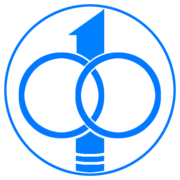
\includegraphics[scale=0.5]{./logo.png}\\[1cm] 
\textsc{\LARGE 乌鲁木齐市第一中学}\\[1.5cm]
\textsc{\Large 研究论文}\\[0.5cm]
{ \huge \bfseries 立体空间中基于计算机视觉与\\几何关系的定位算法}\\[5cm]


% Author and supervisor
\begin{minipage}{0.4\textwidth}
\begin{flushleft} \large
\begin{center}
\emph{作者:}\\
方德治
\end{center}
\end{flushleft}
\end{minipage}
\begin{minipage}{0.4\textwidth}
\begin{flushright} \large
\begin{center}
\emph{指导教师:} \\
卢秀梅
\end{center}
\end{flushright}
\end{minipage}

\vfill

% Bottom of the page
{\large \today}

\end{center}
\end{titlepage}

\begin{abstract}
随着计算机视觉技术的发展,对于实时视频源的计算变得越来越高效。位置信息的获取是计算机视觉领域中较重要的应用之一。室内的环境与室外环境有着诸多不同,其中墙壁对于GPS信号的阻碍作用使得基于卫星的定位在室内变得几乎不可能。因此,为了实现在室内的较精确的定位,需要引入一个全新的绝对参考系。本文提出了一种成本低廉,精度较高,部署方便的定位与追踪算法。
\end{abstract}
\newpage
\tableofcontents
\newpage
\section{总览}
室内的定位系统是近年来的研究热点之一。不少研究团队的研究领域在基于无线信号的定位系统,如基于wifi的室内定位系统\cite{cite1}。然而,由于室内的环境复杂,而无线信号基站的部署成本高昂,这样的定位系统不能得到有效应用。本文中提出了一种基于计算机视觉的定位系统。该系统中使用了普通的网络摄像头作为绝对参考系,从而使得部署成本大大降低。一些基于计算机算法的使用保证了该系统的健壮性与精确性。\\

其中使用的开源库有video4linux\cite{cite2}, OpenCV\cite{cite3}。在开发的过程中使用了Python这一灵活高效的编程语言,使得代码复杂度大大减小,而又不以牺牲较大的性能为代价。

此系统中,共有三个子系统,它们是:
\begin{enumerate}
  \item 视频提取
  \item 小孔摄像机数学模型
  \item Epipolar几何学
\end{enumerate}


\newpage
\section{构造}

\subsection{视频提取}
视频提取系统的主要功能是在视频源中找到某个特定的物体。本例中的物体,指的是有不同颜色的小球。这些小球可以代表要追踪物体的关键部位,从而在后期可以通过几何关系推倒出物体的质心位置与姿态。
视频提取中遇到的主要困难,是不同光照环境下物体颜色的表达不尽相同。不仅如此,由于噪声的大量存在,简单的查找算法不可能胜任这一工作。为此,一个更加复杂的系统被提出了:
\begin{enumerate}
  \item 拍摄:由摄像头中取得符合需求时间戳的图像,
  \item 变换:将图像转化至HSV色彩空间,
  \item 提取:使用阀门来控制颜色数值,使它们落在特定的区间内,再通过频率分布直方图来确定某一像素是否属于追踪的物体,再使用反投影绘制频率图案。
  \item 降噪:使用高斯模糊算法 与 形态学处理算法去除图像中的噪声
  \item 决定:使用Camshift算法来追踪物体的位置
\end{enumerate}
\subsubsection{拍摄}
由于Video4Linux的存在,获取图像是一件十分简单的事。下面给出简单的获取图像的代码:
\lstset{language=python}
\begin{python}
cap = cv2.VideoCapture(source)
img = cap.read()
\end{python}
\subsubsection{变换}
通常的图片文件中表现色彩的方式为RGB方式,然而,RGB方式表示出的图像在不同的光照条件下数值有着显著的不同。与此不同,HSV色彩空间的特性决定了其在此十分适用:其中的V通道表示亮度。在计算时,只忽略V通道中的内容,自然就可得到一个与光照条件无关的表示方法;同时,HSV色彩空间也更为接近人眼对于色彩的表示方法。
HSV色彩空间与RGB色彩空间对应的转化方法如下:\\
\begin{align}
  M &= \operatorname{max}(R, G, B) \\
  m &= \operatorname{min}(R, G, B) \\
  C &= M - m\\
  H^\prime &=
    \begin{cases}
      \mathrm{undefined},        &\mbox{if } C = 0 \\
      \frac{G - B}{C} \;\bmod 6, &\mbox{if } M = R \\
      \frac{B - R}{C} + 2,       &\mbox{if } M = G \\
      \frac{R - G}{C} + 4,       &\mbox{if } M = B
    \end{cases} \\
  H        &= 60^\circ \times H^\prime\\
  V &= M\\
   S &=
    \begin{cases}
      0,           &\mbox{if } C = 0 \\
      \frac{C}{V}, &\mbox{otherwise}
    \end{cases}
\end{align}
可见,在实际的计算结果中,只要有H与S两个通道的数值,就可以决定像素的颜色。没有了V通道使得颜色的亮度不能确定,然而这一点恰恰可以为计算机视觉系统所用。
与之对应的转化代码如下,值得注意的地方是,OpenCV默认使用的是BGR色彩空间,与RGB色彩空间尚有少许不同。
\begin{python}
hsv = cv2.cvtColor(img, cv2.COLOR_BGR2HSV)
\end{python}
\subsubsection{提取}

在提取的过程中一个常见的算法是采用阀门,即为图像设定一个上下极值,使得超出这个区间的数值全部被抛弃,从而获得一个在特定色彩范围内的像素列表。为了使用OpenCV的多线程特性,这个过程的代码如下:
\begin{python}
mask = cv2.inRange( hsv, 
                    np.array((0., 60., 32.)), 
                    np.array((180., 255., 255.))
                    )
\end{python}

然而,简单的阀门却并不对所有情况都有效。甚至可以说,阀门对于大多数情况的处理都是不尽人意的。被追踪的物体由于表面反射光的特性往往呈现出一个范围内的颜色,而不仅仅是某种单一的颜色。这种现象使得阀门处理变得无效了。为了解决这个问题,我们引入色彩分布的直方图。图1是一个简单的频率分布直方图。

\begin{figure}[h]

  \centering
    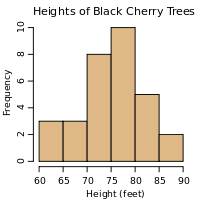
\includegraphics[width=0.2\textwidth]{../Pictures/histogram.JPG}
    \caption{一个简单的频率分布直方图\cite{cite5}}\\
\end{figure}

图中的面积表示出了数据的分布。类似地,我们可以为图像建立相同的直方图。反投影可以使用模型的直方图数据来预测某一像素是否属于追踪的图案中。
考虑一个图像矩阵$M$,其中的每个像素可以被表示为实数对$(H_{i,j},S_{i,j})$。如果我们将两者作为变量,就可以绘制出一副二维的频率分布直方图。其中的图形体积表示的是分布的概率。图2是一个简单的图像直方图,它由样例数据生成。\\
\begin{figure}[h]

  \centering
    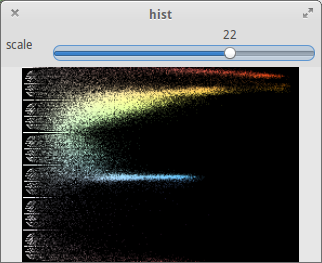
\includegraphics[width=0.3\textwidth]{../Pictures/2dhist.png}
    \caption{一个简单的图像直方图}\\
\end{figure}
在生成这个直方图后,一个像素属于模型的概率可以通过下面的步骤表达:
\begin{enumerate}
  \item 找到一个像素对应的实数对 $(H_{i,j},S_{i,j})$ ,
  \item 在直方图中找到对应的块形,
  \item 由块形的体积确定概率.
\end{enumerate}
在此之后我们就可以使用频率来绘制一副图像。在这图像中每个像素的值代表的是原图片中该像素属于模型的概率。图3是一个反投影的例子:\\
\begin{figure}[h]

  \centering
    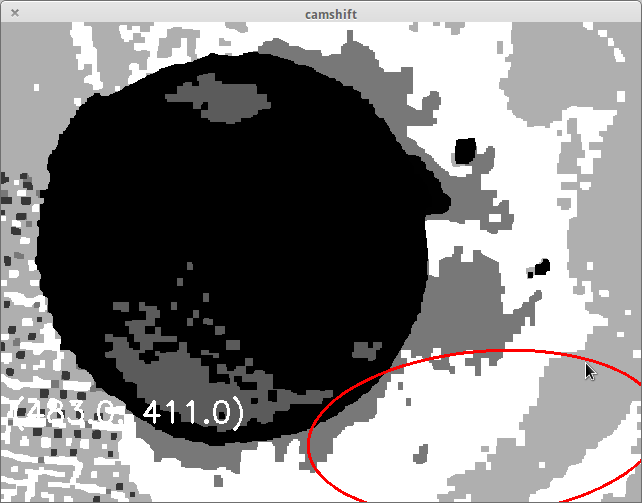
\includegraphics[width=0.5\textwidth]{../Pictures/backproject.png}
    \caption{一个简单的反投影}\\
\end{figure}
\subsubsection{降噪}
在计算出图像的反投影后,理论上就可以计算出物体在图像中的位置了。然而,实际情景中,往往还存在着大量的噪声。这些噪声会对物体的检测进行干扰。为了取得更佳的效果,一个降噪的机制被引入了。

在这个系统中,我们使用了形态学处理。形态学处理中的两种操作,开和闭,能够分别去除图像中较小的噪声,与填补区块中空缺的部分。它们一起恰恰能够满足我们的需求:\\
\begin{figure}[h]

  \centering
    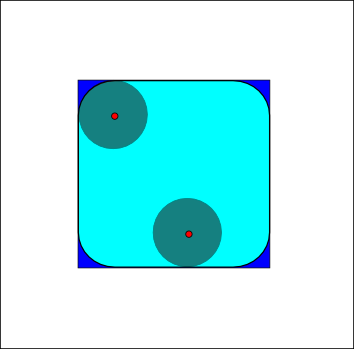
\includegraphics[width=0.3\textwidth]{../Pictures/Opening.png}
    \caption{开 操作的样例\cite{cite7}}\\
\end{figure}
\begin{figure}[h]

  \centering
    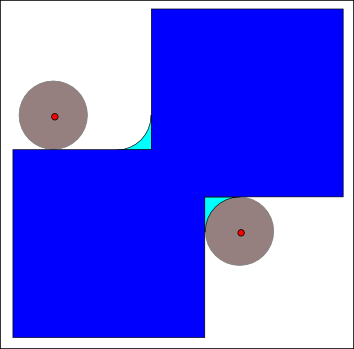
\includegraphics[width=0.3\textwidth]{../Pictures/Closing.png}
    \caption{闭 操作的样例\cite{cite6}}\\
\end{figure}

效果是十分显著的,这个过程中去除了大量的噪声:\\
\begin{figure}[h]

  \centering
    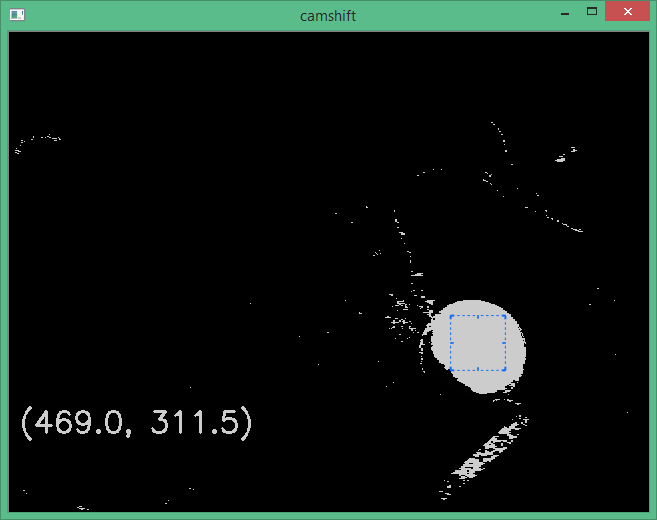
\includegraphics[width=0.3\textwidth]{../Pictures/before.png}
    \caption{形态学处理之前}\\
\end{figure}
\begin{figure}[h!]

  \centering
    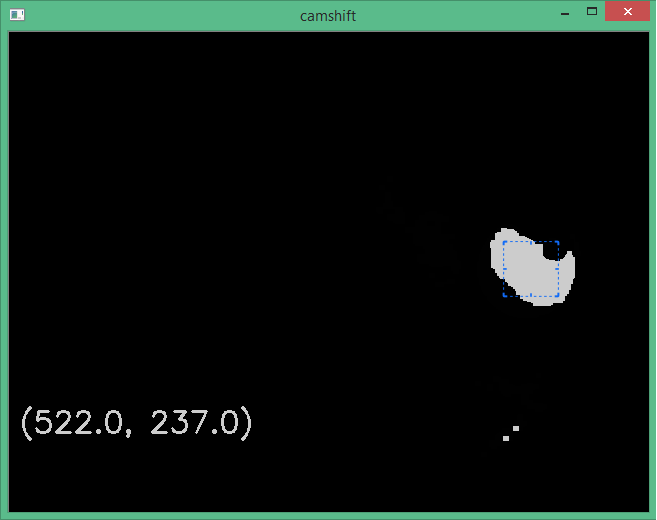
\includegraphics[width=0.3\textwidth]{../Pictures/after.png}
    \caption{形态学处理之后}\\
\end{figure}

然而,使用形态学处理仍然不能满足我们的需求。此时的图像棱角比较明显,为了去除其中模糊的部分,需要引入高斯模糊的算法。
\begin{figure}[h]

  \centering
    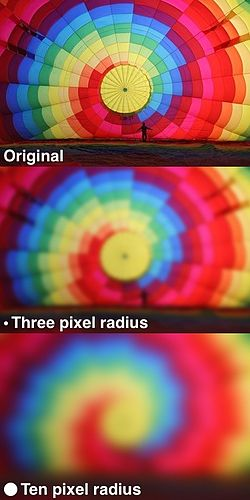
\includegraphics[width=0.3\textwidth]{../Pictures/blur.jpg}
    \caption{高斯模糊的例子}\\
\end{figure}
整个降噪过程的代码表示如下:\newpage
\begin{python}
kernel = np.ones((5,5),np.uint8)
                if MorphOps:
                    prob = cv2.morphologyEx(prob, cv2.MORPH_OPEN, kernel)
                    prob = cv2.morphologyEx(prob, cv2.MORPH_CLOSE, kernel)
                prob = cv2.GaussianBlur(prob,(5,5),0)
\end{python}
\subsubsection{提取}
提取共有两个阶段,它们是:
\begin{enumerate}
  \item 检测
  \item 追踪
\end{enumerate}
其中的区别在于,追踪时物体原有的位置应当是已知的。而这个位置的信息应当由第一阶段,即检测来提供。
检测的过程中,我们寻找图像中与模板内容相似的位置。使用的算法会把模板在图像上移动,并比较模板以下的内容与模板之间的相似度。这个过程的算法如下所示:

\begin{minted}[mathescape,
               linenos,
               numbersep=5pt,
               gobble=2,
               frame=lines,
               framesep=2mm]{python}
  import numpy as np
  import cv2
  import math

  def match(template, image):
    '''
    Match template on image and return the centroid's coord.
    '''

    image = cv2.cvtColor(image, cv2.COLOR_BGR2GRAY)
    template = cv2.cvtColor(template, cv2.COLOR_BGR2GRAY)

    result = cv2.matchTemplate(gray, patch, cv2.TM_CCOEFF_NORMED)
    result = np.abs(result) ** 3
    val, result = cv2.threshold(result, 0.01, 0, cv2.THRESH_TOZERO)

    minVal, maxVal, minLoc, maxLoc = cv2.minMaxLoc(result)

    height, width, depth = template.shape
    x, y = maxLoc
    x += width/2
    y += height/2
      
    return (x,y)
\end{minted}

然而,为了使得图像更加清晰,易于了解,我们还需要在图像上增加一个图形的追踪器。这个过程度算法如下。需要注意的是,这个过程中可能出现图像移动超出边界的情况,对此需要特殊处理。
\begin{minted}[mathescape,
               linenos,
               numbersep=5pt,
               gobble=2,
               frame=lines,
               framesep=2mm]{python}
  import numpy as np
  import cv2
  import math

  def draw_machine_mark(size, location, image):
      '''
      This function draws a machine mark on the image
      '''
      original = cv2.imread("assets/machine.png", -1)

      osize = math.sqrt(original.size)/2
      ratio = size / osize
      height, width, depth = image.shape
      timg = cv2.resize(original, (0,0), fx=ratio, fy=ratio)
      x, y = location 

      image[:] *= 0.8

      x_start = max(0, x - size/2)
      x_end = min(x_start + size, width)
      x_start = min(x_end - size, x_start)
      y_start = max(0, y - size/2)
      y_end = min(y_start + size, height)
      y_start = min(y_end - size, y_start)
      
      roi = image[y_start : y_end, x_start : x_end]
      for c in range(0,3):
          roi[:,:,c] = timg[:,:,c] * (timg[:,:,3] / 255.0) + roi[:,:,c] * (1 - timg[:,:,3] / 255.0) 
      image[y_start : y_end, x_start : x_end] = roi
\end{minted}
下面是一个效果的预览。物体的位置十分清晰可见。\\
\begin{figure}[h!]

  \centering
    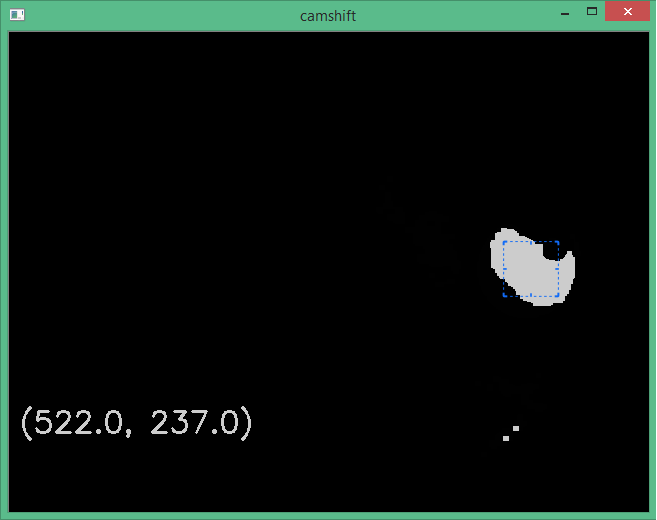
\includegraphics[width=0.5\textwidth]{../Pictures/after.png}
    \caption{Example of tracking effect}\\
\end{figure}

对于Camshift算法,它的本源是MeanShift算法。顾名思义,中值平移算法。它的计算过程如下所示:
\begin{enumerate}
  \item 划定一块区域$S$
  \item 计算$S$中所有点以概率为权的加权平均值
  \item 得到一个新的中心$M_2$
  \item 使得$M_1=M_2$
  \item 将这个值带入下一次迭代
\end{enumerate}
Camshift算法对Meanshift算法的主要改进在于使得搜索空间的位置可以改变了。这样一来随着物体的前后移动,搜索的空间也会随之变化。下面给出一张描述Camshift搜索过程的图解:
\begin{figure}[h!]

  \centering
    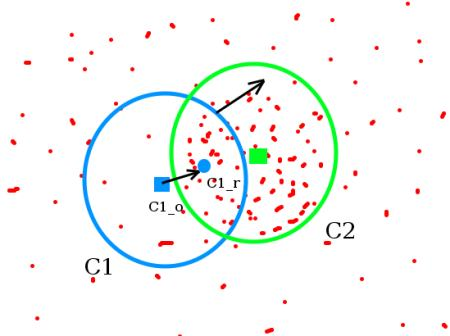
\includegraphics[width=0.5\textwidth]{../Pictures/camshift.jpg}
    \caption{Camshift 算法}\\
\end{figure}
\subsection{小孔摄像机模型}
在视频提取中,我们找到了物体的位置,然而由于摄像头在制造过程中的种种缺陷,我们需要找到一种补偿措施来使得图像不再扭曲。这种模型就是小孔摄像机模型。

一个常见的小孔摄像机模型可以被图11中的几何关系描述:\\
\begin{figure}[h!]

  \centering
    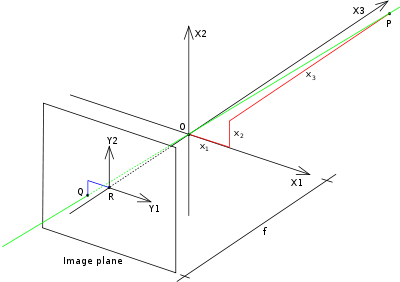
\includegraphics[width=0.5\textwidth]{../Pictures/pin.png}
    \caption{小孔摄像机模型}\\
\end{figure}
\newpage
或者,它也可以被如下的矩阵描述:
$$\begin{pmatrix} y_1 \\ y_2 \\ 1 \end{pmatrix} \sim \begin{pmatrix} 1 & 0 & 0 & 0 \\ 0 & 1 & 0 & 0 \\ 0 & 0 & \frac{1}{f} & 0 \end{pmatrix} \, \begin{pmatrix} x_1 \\ x_2 \\ x_3 \\ 1 \end{pmatrix} $$

用于计算这个矩阵的算法如下:
\begin{python}
chessboard_size = (9, 6)
pattern_points = np.zeros( (np.prod(chessboard_size), 3), np.float32 )
pattern_points[:,:2] = np.indices(chessboard_size).T.reshape(-1, 2)

#Define Cameras
cap0 = cv2.VideoCapture(0)
cap1 = cv2.VideoCapture(1)

obj_points = []
img_points = []
img_points2 = []

chessboard_size = (9, 6)
pattern_points = np.zeros( (np.prod(chessboard_size), 3), np.float32 )
pattern_points[:,:2] = np.indices(chessboard_size).T.reshape(-1, 2)

while True:
	ret, img = cap0.read()
	ret, img2 = cap1.read()
	img = cv2.cvtColor(img, cv2.COLOR_BGR2GRAY)
	img2 = cv2.cvtColor(img2, cv2.COLOR_BGR2GRAY)
	found, corners = cv2.findChessboardCorners(img, chessboard_size)
	found1, corners2 = cv2.findChessboardCorners(img2, chessboard_size)
	if found and found1:
		term = ( cv2.TERM_CRITERIA_EPS + cv2.TERM_CRITERIA_COUNT, 30, 0.1 )
		cv2.cornerSubPix(img, corners, (5, 5), (-1, -1), term)
		cv2.cornerSubPix(img2, corners2, (5, 5), (-1, -1), term)
		vis = cv2.cvtColor(img, cv2.COLOR_GRAY2BGR)
		vis2 = cv2.cvtColor(img2, cv2.COLOR_GRAY2BGR)
		cv2.drawChessboardCorners(vis, chessboard_size, corners, found)
		cv2.drawChessboardCorners(vis2, chessboard_size, corners2, found)
		img=vis
		img2=vis2
		img_points.append(corners.reshape(-1, 2))
		img_points2.append(corners2.reshape(-1, 2))
		obj_points.append(pattern_points)
	cv2.imshow('Image', img)
	cv2.imshow('Image2', img2)
	ch = 0xFF & cv2.waitKey(1)
	if ch == 27:
		break	
retval, cameraMatrix1, distCoeffs1, cameraMatrix2, distCoeffs2, R, T, E, F = cv2.stereoCalibrate(obj_points,
																							img_points,
																							img_points2,
																							(640,480),
																							cameraMatrix1=camera_matrix,
																							distCoeffs1=dist_coefs,
																							cameraMatrix2=camera_matrix,
																							distCoeffs2=dist_coefs,
																							)
\end{python}
通过remap的方式,可以使得原本扭曲的图像恢复原样。下面给出其中的一个操作例子。
\begin{figure}[h!]

  \centering
    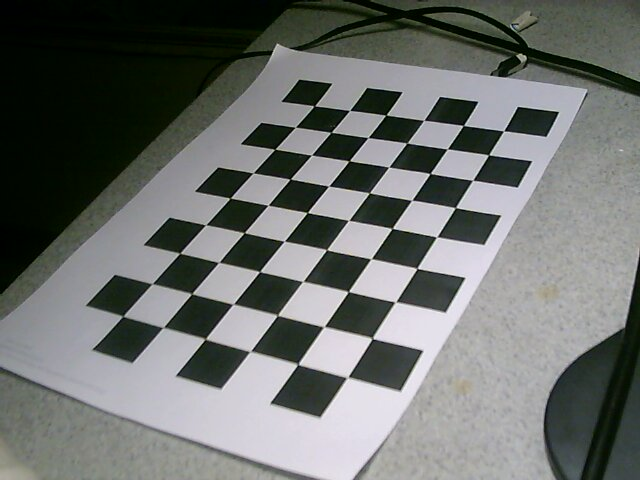
\includegraphics[width=0.5\textwidth]{../src/2014-02-24-225333.jpg}
    \caption{一个处理前的图像}\\
\end{figure}
\begin{figure}[h!]

  \centering
    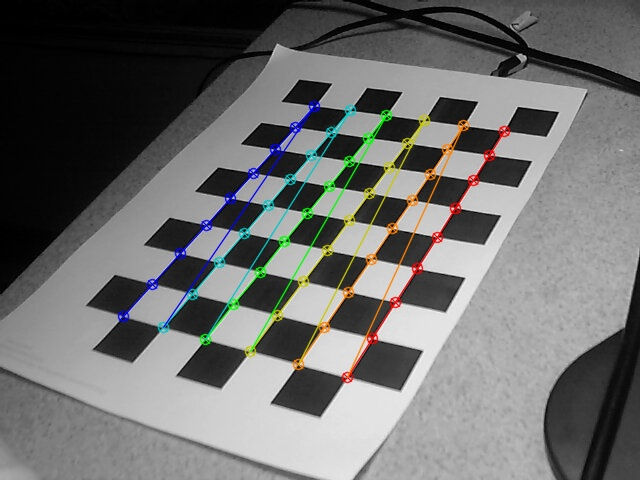
\includegraphics[width=0.5\textwidth]{../src/proc_2014-02-24-225333.jpg}
    \caption{一个经过反扭曲处理的图像}\\
\end{figure}
\subsection{Epipolar几何学}
Epipolar几何学是用来描述三维空间在摄像机平面投影的几何学。其中,物体在两个摄像机图像中的位置可以被转化为空间中的两条直线。图14中展示了一个典型的Epipolar几何学情景:\\
\begin{figure}[h!]

  \centering
    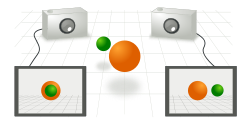
\includegraphics[width=0.5\textwidth]{../Pictures/geo.png}
    \caption{Epipolar几何学}\\
\end{figure}
在这样的情境中,结合上文中的stereoCalibrate函数得到的矩阵Q,可以推算出到坐标的计算方法。
\begin{align}
X &= x_{left} \cdot Q_{0, 0} + Q_{0, 3}\\
Y &= y_{left} \cdot Q_{1, 1} + Q_{1, 3}\\
Z &= Q_{2, 3}\\
W &= (x_{left}-y_{left}) \cdot Q_{3, 2} + Q_{3, 3}\\
X &= \frac{\lambda X}{W}\\
Y &= \frac{\lambda Y}{W}\\
Z &= \frac{\lambda Z}{W}\\
\end{align}
其中,$\lambda$为一个常数,用来表达单位与像素之间的换算关系。
\section{结论}
通过对于计算机视觉系统的探究,我们得到一种成本低廉,精确度高的定位算法。该算法对于无人机在室内的定位犹为重要,我们的室内完全自动飞行四轴飞行器也已在开发中。这一定位算法仍有许多不足之处,但是我们有理由相信,他们都会被不断改进。Knowledge is the undoubtable ultimate power.
\section{附录}
\newpage
\appendix
\section{\\Camshift.py} \label{App:AppendixA}
\begin{python}
#!/usr/bin/env python

import numpy as np
import cv2
import video
from utils import mark

size_treshold = 4
side_inc = 2
size_maxium = 256
flag= True
MorphOps = False
Channel = False
Realtime = False
Update = False

def abs(n):
    if n>0:
        return n
    return -n

def get_window_size(window):
    x0, y0, x1, y1 = window
    size = abs(x1) * abs(y1)
    return size

def get_increased_window(window):
    xx0, yy0, xx1, yy1 = window
    xx0 -= side_inc
    yy0 -= side_inc
    xx1 += side_inc
    yy1 += side_inc
    xx0, yy0, xx1, yy1 = max(0, xx0), max(0, yy0), min(size_maxium, max(1, xx1)), min(size_maxium, max(1, yy1))# Make the square's size at least 1 pixel.
    new_window = (xx0, yy0, xx1, yy1)
    return new_window

class App(object):
    def __init__(self, video_src):
        self.cam = video.create_capture(1)
        ret, self.frame = self.cam.read()
        cv2.namedWindow('camshift')
        cv2.setMouseCallback('camshift', self.onmouse)
        self.mouse_state = 0
        self.selection = None
        self.drag_start = None
        self.tracking_state = 0
        self.show_backproj = False

    def onmouse(self, event, x, y, flags, param):
        x, y = np.int16([x, y]) # BUG
        #print (x,y)
        debug={}
        bkp=flags
        if event == cv2.EVENT_LBUTTONDOWN:
            #print (x,y)
            self.drag_start = (x, y)
            self.tracking_state = 0
            self.mouse_state = 1
        elif event == cv2.EVENT_MOUSEMOVE:
            if self.mouse_state:
                h, w = self.frame.shape[:2]
                xo, yo = self.drag_start
                x0, y0 = np.maximum(0, np.minimum([xo, yo], [x, y]))
                x1, y1 = np.minimum([w, h], np.maximum([xo, yo], [x, y]))
                #print (x0,y0,x1,y1)
                self.selection = None
                if x1-x0 > 0 and y1-y0 > 0:
                    self.selection = (x0, y0, x1, y1)
                    #print self.selection
        elif event == cv2.EVENT_LBUTTONUP:
            self.mouse_state = 0
            self.drag_start = None
            flag= False
            if self.selection is not None:
                self.tracking_state = 1
    def show_hist(self):
        bin_count = self.hist.shape[0]
        bin_w = 24
        img = np.zeros((256, bin_count*bin_w, 3), np.uint8)
        for i in xrange(bin_count):
            h = int(self.hist[i])
            cv2.rectangle(img, (i*bin_w+2, 255), ((i+1)*bin_w-2, 255-h), (int(180.0*i/bin_count), 255, 255), -1)
        img = cv2.cvtColor(img, cv2.COLOR_HSV2BGR)
        cv2.imshow('hist', img)

    def run(self):
        global Update
        global MorphOps
        global Channel
        global Realtime
        while True:

            ret, self.frame = self.cam.read()
            vis = self.frame.copy()
            hsv = cv2.cvtColor(self.frame, cv2.COLOR_BGR2HSV)
            mask = cv2.inRange(hsv, np.array((0., 60., 32.)), np.array((180., 255., 255.)))
            mask = cv2.inRange(hsv, np.array((0., 0., 0.)), np.array((180., 255., 255.)))
            if self.selection:
                x0, y0, x1, y1 = self.selection
                self.track_window = (x0, y0, x1-x0, y1-y0)
                hsv_roi = hsv[y0:y1, x0:x1]
                mask_roi = mask[y0:y1, x0:x1]

                if Channel:
                    hist = cv2.calcHist( [hsv_roi], [0,1], mask_roi, [16,5], [0, 180, 0 ,256] )
                else:
                    hist = cv2.calcHist( [hsv_roi], [0], mask_roi, [16], [0, 180] )
                cv2.normalize(hist, hist, 0, 255, cv2.NORM_MINMAX)
                self.hist = hist.reshape(-1)
                self.show_hist()

                vis_roi = vis[y0:y1, x0:x1]
                cv2.bitwise_not(vis_roi, vis_roi)
                vis[mask == 0] = 0

            if self.tracking_state == 2:
                if Channel:
                    prob = cv2.calcBackProject([hsv], [0,1], self.hist, [0, 180, 0, 256], 1)
                else:
                    prob = cv2.calcBackProject([hsv], [0], self.hist, [0, 180], 1)
                prob &= mask
                term_crit = ( cv2.TERM_CRITERIA_EPS | cv2.TERM_CRITERIA_COUNT, 10, 1 )
                self.previous_window = self.track_window
                kernel = np.ones((5,5),np.uint8)
                if MorphOps:
                    prob = cv2.morphologyEx(prob, cv2.MORPH_OPEN, kernel)
                    prob = cv2.morphologyEx(prob, cv2.MORPH_CLOSE, kernel)
                prob = cv2.GaussianBlur(prob,(5,5),0)

                track_box, self.track_window = cv2.CamShift(prob, self.track_window, term_crit)
                if get_window_size(self.track_window) <= size_treshold:
                    self.track_window = get_increased_window(self.previous_window)
                    self.tracking_state = 2
                else :
                    self.tracking_state = 1
                font = cv2.FONT_HERSHEY_SIMPLEX
                print "Target Missing."
                cv2.putText(vis,'Target Missing',(10,400), font, 1,(255,255,255),2,1)

            if self.tracking_state == 1:
                self.selection = None
                if Channel:
                    prob = cv2.calcBackProject([hsv], [0,1], self.hist, [0, 180, 0, 256], 1)
                else:
                    prob = cv2.calcBackProject([hsv], [0], self.hist, [0, 180], 1)
                prob &= mask
                term_crit = ( cv2.TERM_CRITERIA_EPS | cv2.TERM_CRITERIA_COUNT, 10, 1 )
                self.previous_window = self.track_window
                kernel = np.ones((5,5),np.uint8)
                if MorphOps:
                    prob = cv2.morphologyEx(prob, cv2.MORPH_OPEN, kernel)
                    prob = cv2.morphologyEx(prob, cv2.MORPH_CLOSE, kernel)
                prob = cv2.GaussianBlur(prob,(5,5),0)
                track_box, self.track_window = cv2.CamShift(prob, self.track_window, term_crit)
                if get_window_size(self.track_window) <= size_treshold:
                    self.track_window = get_increased_window(self.previous_window)
                    self.tracking_state = 2
                if self.show_backproj:
                    vis[:] = prob[...,np.newaxis]
                xx0, yy0, xx1, yy1 = self.track_window
                img_roi = self.frame[yy0 : yy0 + yy1, xx0 : xx0 + xx1]
                cv2.imshow("Tracking Window",img_roi)
                if get_window_size(self.track_window) >= size_treshold and Update:
                    self.bkp=self.hist
                    font = cv2.FONT_HERSHEY_SIMPLEX
                    cv2.putText(vis,'Updating...',(10,200), font, 1,(255,255,255),2,1)
                    xx0, yy0, xx1, yy1 = self.track_window
                    xx1 /= 3
                    yy1 /= 3
                    xx0 += xx1
                    yy0 += yy1
                    if xx1 > 0 and yy1 > 0:
                        print self.track_window
                        hsv_roi = hsv[yy0 : yy0 + yy1, xx0 : xx0 + xx1]
                        mask_roi = mask[yy0 : yy0 + yy1 , xx0 : xx0 + xx1]
                        cv2.imshow("Tracking Window",hsv_roi)
                        hist = cv2.calcHist( [hsv_roi], [0], mask_roi, [16], [0, 180] )
                        cv2.normalize(hist, hist, 0, 255, cv2.NORM_MINMAX)
                        print cv2.compareHist(hist.reshape(-1), self.bkp, 0)
                        self.hist = hist.reshape(-1)
                    self.show_hist()
                    if not Realtime:
                        Update = not Update
                font = cv2.FONT_HERSHEY_SIMPLEX
                cv2.putText(vis,str(track_box[0]),(10,400), font, 1,(255,255,255),2,1)
                print str(track_box[0])
                #try: cv2.ellipse(vis, track_box, (0, 0, 255), 2)
                #except: print track_box
                mark.draw_machine_mark(60, track_box[0], vis)

            #cv2.imshow('Original Footage',self.frame)
            if flag:
                cv2.imshow('camshift', vis)

            ch = 0xFF & cv2.waitKey(5)
            if ch == 27:
                break
            if ch == ord('b'):
                self.show_backproj = not self.show_backproj
            if ch == ord('m'):
                MorphOps = not MorphOps
            if ch == ord('c'):
                Channel = not Channel
            if ch == ord('u'):
                Update = not Update
            if ch == ord('r'):
                Realtime = not Realtime
        cv2.destroyAllWindows()


if __name__ == '__main__':
    import sys
    try: video_src = sys.argv[1]
    except: video_src = 0
    print __doc__
    App(video_src).run()

\end{python}
\newpage
\section{Bi-calibration.py} \label{App:AppendixB}
% the \\ insures the section title is centered below the phrase: Appendix B
\begin{python}
import numpy as np
import cv2
import os
import sys, getopt
from glob import glob

img_set = '2*.jpg'
img_names = glob(img_set)

chessboard_size = (9, 6)
pattern_points = np.zeros( (np.prod(chessboard_size), 3), np.float32 )
pattern_points[:,:2] = np.indices(chessboard_size).T.reshape(-1, 2)

obj_points = []
img_points = []
h, w = 0, 0
for name in img_names:
    print 'Detecting chessboard on %s...' % name,
    img = cv2.imread(name, 0)
    h, w = img.shape[:2]
    found, corners = cv2.findChessboardCorners(img, chessboard_size)
    if found:
        term = ( cv2.TERM_CRITERIA_EPS + cv2.TERM_CRITERIA_COUNT, 30, 0.1 )
        cv2.cornerSubPix(img, corners, (5, 5), (-1, -1), term)
        vis = cv2.cvtColor(img, cv2.COLOR_GRAY2BGR)
        cv2.drawChessboardCorners(vis, chessboard_size, corners, found)
        cv2.imshow('Corners', vis)
        cv2.imwrite('proc_'+name,vis)
        cv2.waitKey(200)
    if not found:
        print 'chessboard not found'
        continue
    img_points.append(corners.reshape(-1, 2))
    obj_points.append(pattern_points)

    print 'ok'

rms, camera_matrix, dist_coefs, rvecs, tvecs = cv2.calibrateCamera(obj_points, img_points, (w, h))
print "RMS:", rms
print "camera matrix:\n", camera_matrix
print "distortion coefficients: ", dist_coefs.ravel()
img = cv2.imread('1.jpg')
h,  w = img.shape[:2]
newcameramtx, roi=cv2.getOptimalNewCameraMatrix(camera_matrix,dist_coefs,(w,h),1,(w,h))
# undistort
dst = cv2.undistort(img, camera_matrix, dist_coefs, None, newcameramtx)

# crop the image
x,y,w,h = roi
dst = dst[y:y+h, x:x+w]
cv2.imwrite('calibresult.png',dst)

chessboard_size = (9, 6)
pattern_points = np.zeros( (np.prod(chessboard_size), 3), np.float32 )
pattern_points[:,:2] = np.indices(chessboard_size).T.reshape(-1, 2)

#Define Cameras
cap0 = cv2.VideoCapture(0)
cap1 = cv2.VideoCapture(1)

obj_points = []
img_points = []
img_points2 = []

chessboard_size = (9, 6)
pattern_points = np.zeros( (np.prod(chessboard_size), 3), np.float32 )
pattern_points[:,:2] = np.indices(chessboard_size).T.reshape(-1, 2)

while True:
	ret, img = cap0.read()
	ret, img2 = cap1.read()
	img = cv2.cvtColor(img, cv2.COLOR_BGR2GRAY)
	img2 = cv2.cvtColor(img2, cv2.COLOR_BGR2GRAY)
	found, corners = cv2.findChessboardCorners(img, chessboard_size)
	found1, corners2 = cv2.findChessboardCorners(img2, chessboard_size)
	if found and found1:
		term = ( cv2.TERM_CRITERIA_EPS + cv2.TERM_CRITERIA_COUNT, 30, 0.1 )
		cv2.cornerSubPix(img, corners, (5, 5), (-1, -1), term)
		cv2.cornerSubPix(img2, corners2, (5, 5), (-1, -1), term)
		vis = cv2.cvtColor(img, cv2.COLOR_GRAY2BGR)
		vis2 = cv2.cvtColor(img2, cv2.COLOR_GRAY2BGR)
		cv2.drawChessboardCorners(vis, chessboard_size, corners, found)
		cv2.drawChessboardCorners(vis2, chessboard_size, corners2, found)
		img=vis
		img2=vis2
		img_points.append(corners.reshape(-1, 2))
		img_points2.append(corners2.reshape(-1, 2))
		obj_points.append(pattern_points)
	cv2.imshow('Image', img)
	cv2.imshow('Image2', img2)
	ch = 0xFF & cv2.waitKey(1)
	if ch == 27:
		break	
retval, cameraMatrix1, distCoeffs1, cameraMatrix2, distCoeffs2, R, T, E, F = cv2.stereoCalibrate(obj_points,
																							img_points,
																							img_points2,
																							(640,480),
																							cameraMatrix1=camera_matrix,
																							distCoeffs1=dist_coefs,
																							cameraMatrix2=camera_matrix,
																							distCoeffs2=dist_coefs,
																							)
print "-cameraMatrix1:"
print cameraMatrix1
np.save('cameraMatrix1.npy', cameraMatrix1)
print "-distCoeffs1:"
print distCoeffs1
np.save('distCoeffs1.npy', distCoeffs1)
print "-cameraMatrix2:"
print cameraMatrix2
np.save('cameraMatrix2.npy', cameraMatrix2)
print "-distCoeffs2:"
print distCoeffs2
np.save('distCoeffs2.npy', distCoeffs2)
print "-R:"
print R
np.save('R.npy', R)
print "-T:"
print T
np.save('T.npy', T)
print "-E:"
print E
np.save('E.npy', E)
print "-F:"
print F
np.save('F.npy', F)


\end{python}

\newpage
\begin{thebibliography}{1}

\bibitem{cite1}
  Vladimir Maximov and Oleg Tabarovsky, LLC RTLS, Moscow, Russia (2013). Survey of Accuracy Improvement Approaches for Tightly Coupled ToA/IMU Personal Indoor Navigation System. Proceedings of International Conference on Indoor Positioning and Indoor Navigation, October 2013, Montbeliard, France
\bibitem{cite2}
Video4Linux, http://linuxtv.org
\bibitem{cite3}
OpenCV, http://opencv.org
\bibitem{cite4}
Computer Vision Face Tracking For Use in a Perceptual User Interface, 
Gary R. Bradski, Microcomputer Research Lab, Santa Clara, CA, Intel Corporation
\bibitem{cite5}
  Wikipedia ,
  \emph{File:Black cherry tree histogram.svg}.
  \url{http://en.wikipedia.org/wiki/File:Black_cherry_tree_histogram.svg}
\bibitem{cite6}
  Wikipedia ,
  \emph{File:Closing.png}.
  \url{http://en.wikipedia.org/wiki/File:Closing.png}
\bibitem{cite7}
  Wikipedia ,
  \emph{File:Opening.png}.
  \url{http://en.wikipedia.org/wiki/File:Opening.png}
\bibitem{cite8}
  Wikipedia ,
  \emph{File:Pinhole.svg}.
  \url{http://en.wikipedia.org/wiki/File:Pinhole.svg}
\end{thebibliography}

\end{document}
